\documentclass[12pt,letterpaper]{article}
\usepackage[utf8]{inputenc}
\usepackage[spanish,es-tabla]{babel}
\decimalpoint
\let\cleardoublepage\clearpage
% \usepackage[bitstream-charter]{mathdesign} 
% \usepackage[T1]{fontenc}
% \newcommand{\selectSans}{\usefont{T1}{qhv}{m}{n}\selectfont} % sans-serif TeX Gyre Heros font
\usepackage{amsmath}
\usepackage{amsfonts}
\usepackage{amssymb}
% \usepackage[T1]{fontspec}
\usepackage{color}
\usepackage{graphicx}
\usepackage{makeidx}
\makeindex
\usepackage{anysize}
\usepackage{anyfontsize}
\usepackage{pdfpages}
\usepackage[x11names,table]{xcolor}
\usepackage{tikz}
\usepackage{tcolorbox}
\tcbuselibrary{skins,breakable,listings,theorems}
\usepackage[hidelinks]{hyperref}
\usepackage[labelfont=bf]{caption}
\captionsetup[table]{labelsep=space}
\captionsetup[figure]{labelsep=space}
\usepackage{listings}
\usepackage{array,ragged2e}
\usepackage{multirow}
\usepackage[left=2.5cm,top=2cm,right=2.5cm,bottom=2cm]{geometry}
\setlength{\parindent}{0cm}
% \usepackage[printwatermark]{xwatermark}
% \newwatermark[allpages,color=gray!10,angle=45,scale=3,xpos=0,ypos=0]{Borrador}

\tcbset{colback=green!5!white, colframe=gray!10!black, coltitle=green!20!black, 
fonttitle=\bfseries, colbacktitle=white, coltext=gray!30!black}
\addto\captionsspanish{
  \renewcommand{\figurename}{{\bf Figura}}% 
}
\addto\captionsspanish{
  \renewcommand{\chaptername}{{\bf}}% 
}

\usepackage{epigraph}
\usepackage{fontawesome}
\usepackage[Bjornstrup]{fncychap}

% \renewcommand{\familydefault}{\sfdefault}

% Colores
\definecolor{verdep}{RGB}{166,206,58}
\definecolor{ccap}{RGB}{10,10,50}
\definecolor{csec}{RGB}{50,50,100}
\definecolor{csubsec}{RGB}{80,80,120}
\definecolor{header_table_color}{RGB}{200,255,180}
\definecolor{info_color}{RGB}{100,100,200}
\definecolor{csol}{rgb}{0.2,0.8,0.1}
\definecolor{backcode}{rgb}{0.98,0.98,0.99}
\definecolor{crule}{rgb}{0.9,0.9,0.9}
\definecolor{dkgreen}{rgb}{0,0.6,0}
\definecolor{gray}{rgb}{0.5,0.5,0.5}
\definecolor{mauve}{rgb}{0.58,0,0.82}


\newtcolorbox{ejemplo}[2][]
{
  breakable,
  colframe = gray!50,
  colback  = gray!0,
  coltitle = gray!20!black,
  title    =  \faEdit \hspace{5 mm} #2,
}

\newtcolorbox{informacion}[2][]
{
  breakable,
  colframe = blue!5!white,
  colback  = blue!5!white,
  coltitle = blue!80!black,
  title    = \faInfo \hspace{5 mm} #2,
}

\newtcolorbox{recomendacion}[2][]
{
  breakable,
  colframe = green!25,
  colback  = green!10,
  coltitle = green!20!black,
  title    = #2,
}

\newcolumntype{P}[1]{>{\centering\arraybackslash}m{#1}}
\newcommand{\ccol}{>{\centering\tt\arraybackslash}}

% Nuevos comandos

\usepackage{titlesec}%--
% \newcommand{\hsp}{\hspace{5pt}}
% \titleformat{\chapter}[hang]{\huge\bfseries\color{ccap}}
% {\color{verdep}{\vrule height 2.5cm width 1mm}\hsp{\fontsize{100}{5}\selectfont\thechapter}\hsp%
% {\vrule height 2.5cm width 1mm}\hsp{\fontsize{30}{5}\selectfont}}{5pt}{\huge\bfseries}

\titleformat{\section}[hang]{\normalfont\color{csec}}%
{\filright\large\enspace\thesection\enspace}%
{8pt}{\Large\bfseries\filright}%

\titleformat{\subsection}[hang]{\normalfont\color{csec}}%
{\filright\large\enspace\thesubsection\enspace}%
{8pt}{\large\bfseries\filright}%

% Code
\lstnewenvironment{matlab}{\lstset{frame=single,
  frameround=tttt,
  backgroundcolor=\color{backcode},
  rulecolor=\color{crule},
  language=matlab,
  aboveskip=5mm,
  belowskip=5mm,
  showstringspaces=false,
  columns=flexible,
  basicstyle={\small\ttfamily},
  numbers=none,
  numberstyle=\tiny\color{gray},
  keywordstyle=\color{blue},
  commentstyle=\color{dkgreen},
  stringstyle=\color{mauve},
  breaklines=true,
  breakatwhitespace=true,
  tabsize=4,
  extendedchars=true,
  inputencoding=utf8,
  literate=%
  {°}{{\,\,$^\circ$\,\,}}1
  {á}{{\'a}}1
  {é}{{\'e}}1
  {í}{{\'i}}1
  {ó}{{\'o}}1
  {ú}{{\'u}}1
  {Á}{{\'A}}1
  {É}{{\'E}}1
  {Í}{{\'I}}1
  {Ó}{{\'O}}1
  {Ú}{{\'U}}1
}}{}


\author{{\small Pedro Jorge De Los Santos}}
\title{
\vspace{-20mm}
{\normalsize Instituto Tecnológico de Celaya}\\[-2mm]
{\normalsize Departamento de Ingeniería Mecánica}\\[-2mm]
{\normalsize Mecánica de Materiales / Enero-Junio 2017} \\[-2mm]
{\normalsize\bfseries Instalando Python y las bibliotecas a utilizar}
}
\date{}
% =================================================================
% =================================================================
%                              CONTENIDO
% =================================================================
% =================================================================

\begin{document}
\maketitle

\section{¿Qué es Python?}

Python es un lenguaje de programación de alto nivel, de propósito general, que es ampliamente utilizado en computación científica e ingeniería. Como un lenguaje de uso general, Python no fue diseñado específicamente para la computación numérica, pero muchas de sus características lo hacen muy adecuado para esta tarea. \\

Python posee una licencia de código abierto y una extensa comunidad que posibilita disponer de una cantidad enorme de bibliotecas destinadas 
a resolver tareas más específicas. \\

Para nuestros propósitos, las librerías que se usarán están orientadas a la computación técnico-científica, sobre todo algebra simbólica, análisis numérico y 
visualización gráfica. De manera general, las librerías a utilizar son las que se listan a continuación:

\begin{itemize}
\item NumPy (\textit{Manejo de estructuras matriciales})
\item Matplotlib (\textit{Visualización gráfica 2D})
\item SymPy (\textit{Computación simbólica})
\item SciPy (\textit{Colección de algoritmos de ingeniería})
\item Jupyter (\textit{Aplicación web que permite crear y compartir documentos que contienen código interactivo, ecuaciones, texto y gráficos.})
\end{itemize}


\section{Descarga e instalación de Python}

Cuando se utiliza Python en ingeniería lo más recomendable es instalar la distribución \textbf{Anaconda}, que básicamente contiene la instalación base 
de Python más las librerías más relevantes en el ámbito de ingeniería, incluyendo todas las que se listan en la sección anterior. La 
distribución \textbf{Anaconda} se puede descargar desde la página de Continuum Analytics: \\

\url{https://www.continuum.io/downloads} \\

La URL anterior le llevará a una pantalla como la que muestra en la figura \ref{fig:anaconda_download}, en donde déberá seleccionar/descargar el instalador 
para la versión 2.7 de Python y por supuesto, la arquitectura correspondiente de su PC (32-bit/64-bit).

\begin{center}
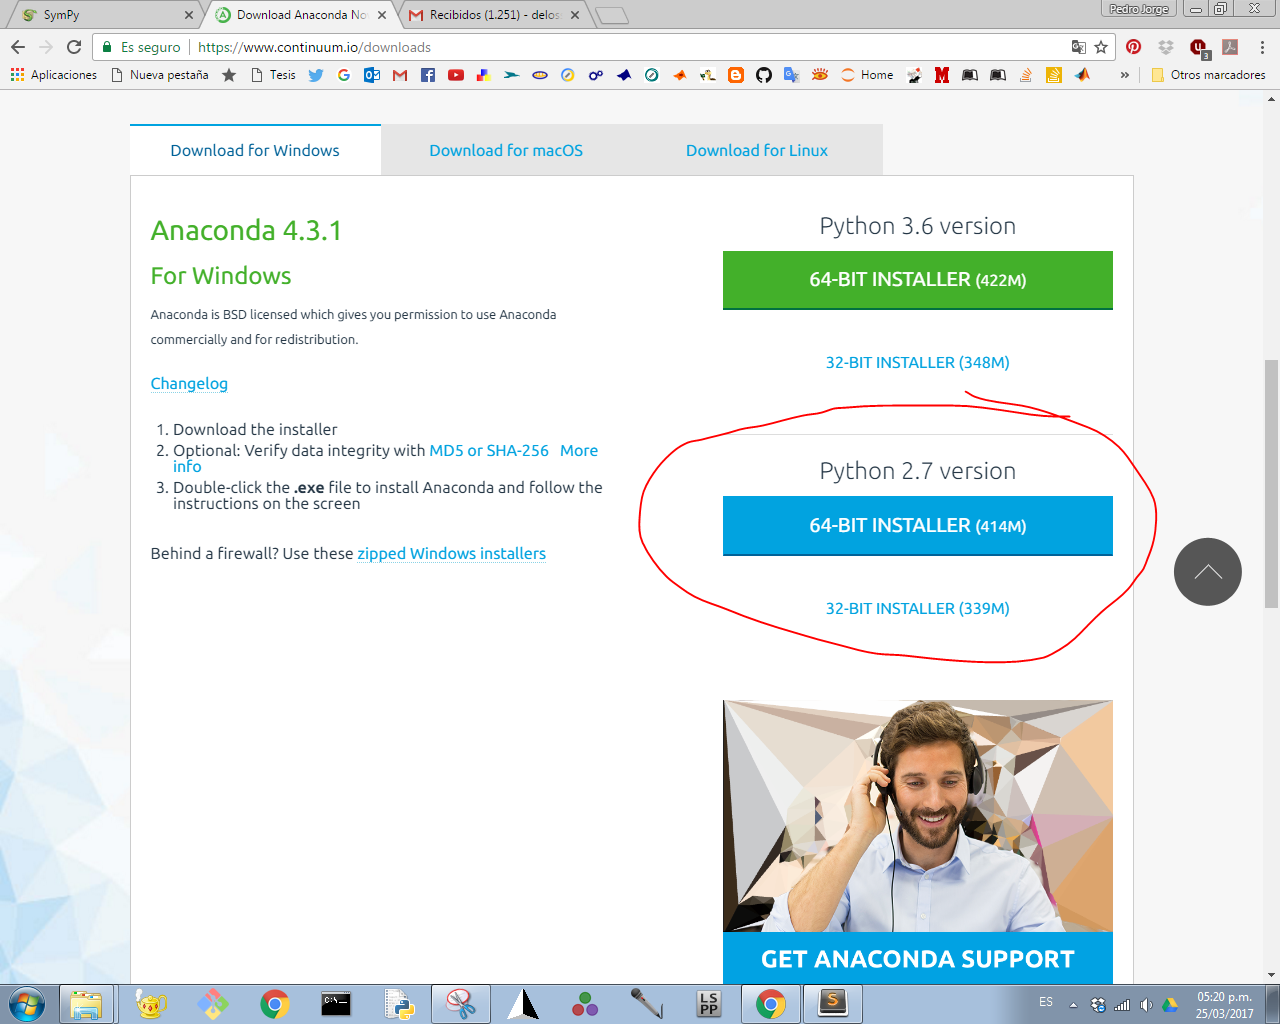
\includegraphics[width=0.65\textwidth]{img/anaconda_download.PNG}
\captionof{figure}{Página de descargas de Anaconda}
\label{fig:anaconda_download}
\end{center}

La instalación es trivial, sólo debe seguir las instrucciones y completarla.


\section{Ejecución de Python}

Para comprobar que Python ha sido instalado correctamente y que el directorio de instalación ha sido agregado al \textit{path} del 
sistema operativo, abra una consola y escriba {\bf\tt python}, como se muestra en la figura \ref{fig:consola_test}. Si le 
aparece un mensaje como el mostrado en la figura \ref{fig:consola_ok}, entonces Python está funcionando de manera correcta. 
En cambio, si le muestra un mensaje como el de la figura \ref{fig:consola_no_ok}, entonces deberá modificar el \textit{path} como 
se explica en el siguiente video: \url{https://www.youtube.com/watch?v=dU_ca27EGT8}. Las carpetas que debe agregar al \textit{path} son 
\verb|C:\Python27| y \verb|C:\Python27\Scripts|.


\begin{center}
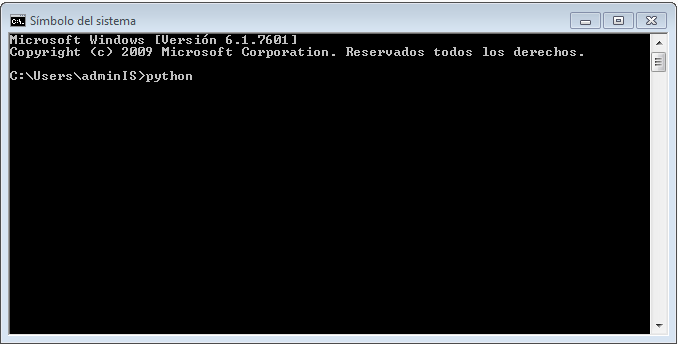
\includegraphics[width=0.65\textwidth]{img/consola_test.PNG}
\captionof{figure}{Testeando en la consola}
\label{fig:consola_test}
\end{center}

\begin{center}
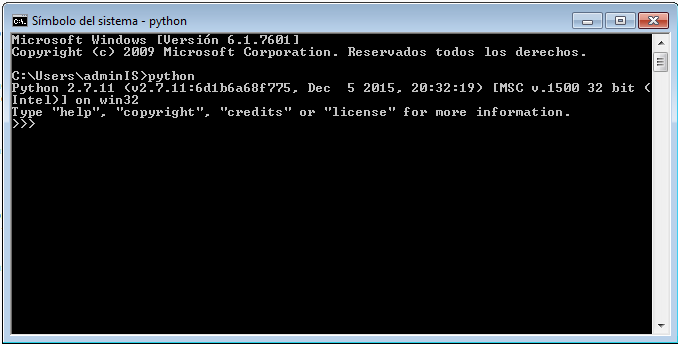
\includegraphics[width=0.65\textwidth]{img/consola_ok.PNG}
\captionof{figure}{Python funcionando}
\label{fig:consola_ok}
\end{center}

\begin{center}
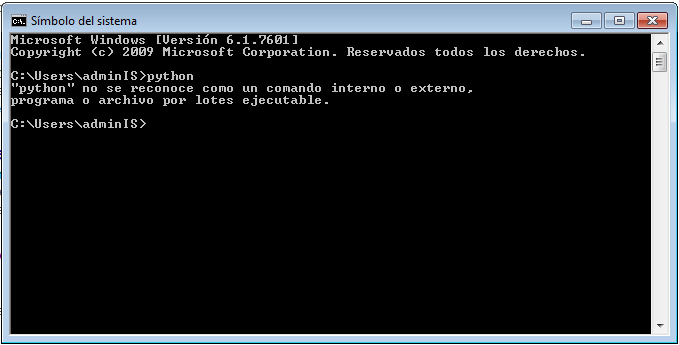
\includegraphics[width=0.65\textwidth]{img/consola_no_ok.PNG}
\captionof{figure}{Python sin funcionar}
\label{fig:consola_no_ok}
\end{center}


\section{Ejecución de Jupyter}

Jupyter es una aplicación web que permite crear y compartir documentos con código Python interactivo, gráficas, ecuaciones y 
texto formateado mediante el lenguaje de marcado Markdown.\\

Para abrir la aplicación deberá teclear en una consola la instrucción {\bf\tt jupyter notebook} como se muestra en 
la figura \ref{fig:jupyter} y enseguida se abrirá una interfaz como la mostrada en la figura \ref{fig:jupyter_interfaz}.

\begin{center}
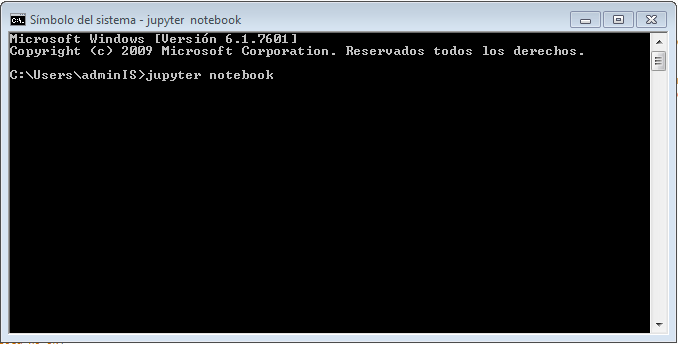
\includegraphics[width=0.65\textwidth]{img/jupyter.PNG}
\captionof{figure}{Ejecutando Jupyter}
\label{fig:jupyter}
\end{center}


\begin{center}
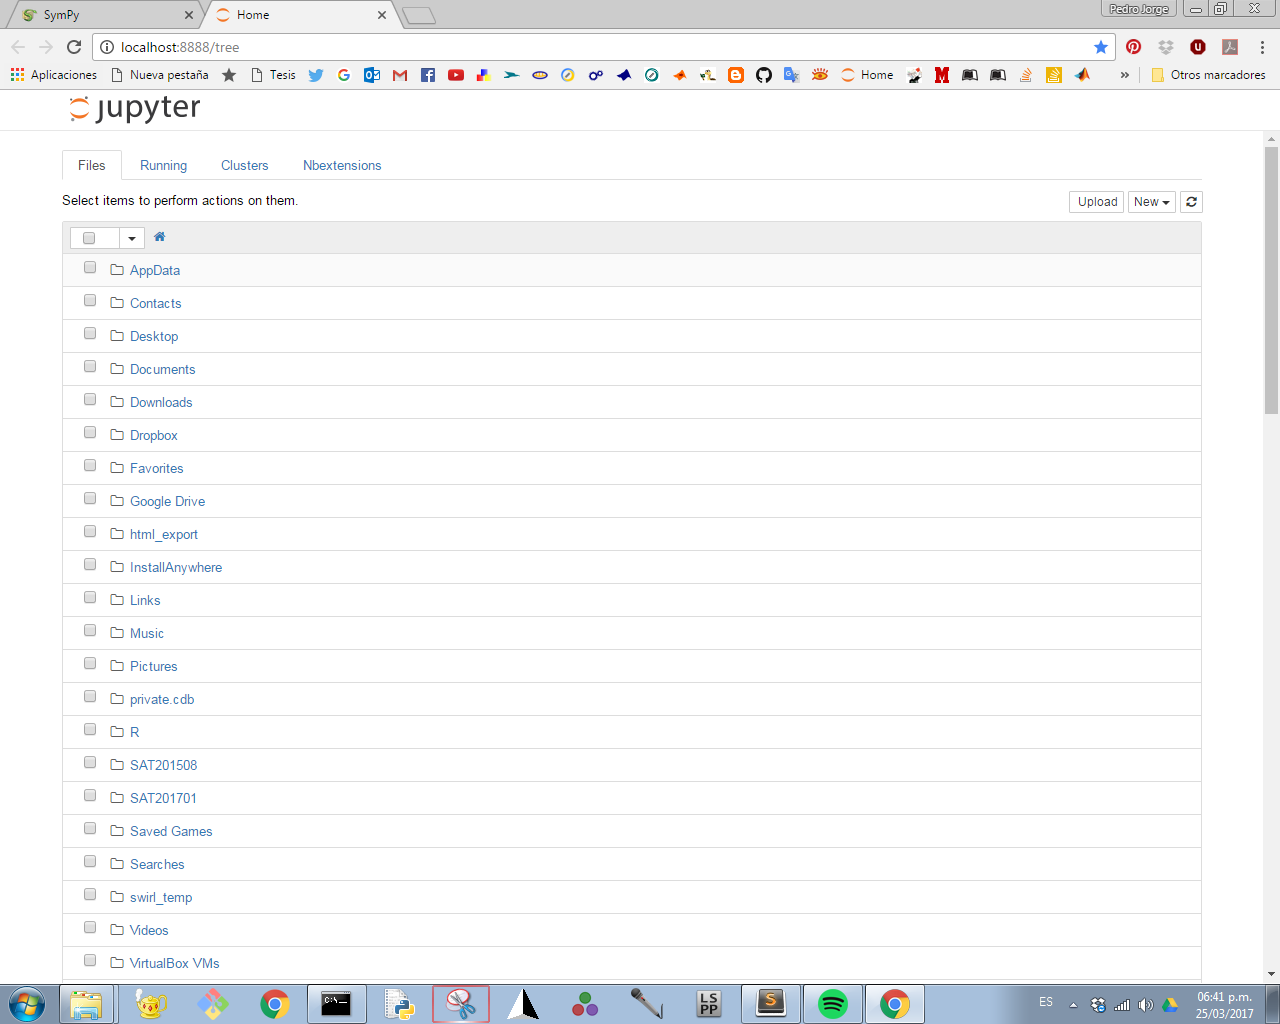
\includegraphics[width=0.65\textwidth]{img/jupyter_interfaz.PNG}
\captionof{figure}{Interfaz de Jupyter}
\label{fig:jupyter_interfaz}
\end{center}


\section{Curso de Python para ingenieros}

El siguiente es un link a un curso de Python para ingenieros por la Universidad de Alicante, en el cual se hace 
una excelente introducción al uso de Python y Jupyter para cuestiones relacionadas con la ingeniería. \\

\url{https://www.youtube.com/watch?v=ox09Jko1ErM&list=PLGBbVX_WvN7bMwYe7wWV5TZt1a58jTggB}




\end{document}